\section{Simulation Results}
\label{sec:simulation}

We evaluate nine questions: (Q1) does the empirical operating point match the
optimal belief threshold predicted by Theorem~\ref{thm:tradeoff}; (Q2) does
the continuous belief-map state confer the access-side advantage implied by
Proposition~\ref{thm:sufficiency}; (Q3) does the distributional CVaR
constraint reduce collision tail risk (Theorem~\ref{thm:cvar}); (Q4) what does
each component (M1/M2/M3) contribute; (Q5) is access performance governed by
\emph{frequency}- rather than temporal-localization accuracy, as the frame
structure of Section~\ref{subsec:access} predicts; (Q6) does sharper
frequency localization translate into better access, as predicted by the
localization-error model \eqref{eq:loc_to_cell} and Corollary~\ref{cor:loc};
(Q7) is the \emph{complete} error-propagation chain
$\eloc\!\to\!(\Pmd,\Pfa)\!\to\!\Pcol\!\to\!\thru$ borne out at every link, not
just its endpoints; (Q8) is the access advantage monotone in the
\emph{information richness} of the state representation, as
Proposition~\ref{thm:sufficiency} implies, rather than an artifact of feature
engineering; and (Q9) does the belief-map advantage \emph{generalize} across
stressed environments (traffic burstiness, PU density, and sensing SNR)?
For Q5--Q9 we use a localization-aware variant of the environment in which the
belief map is rendered from \emph{estimated PU frequency intervals} with a
controllable IoU error, so that cell-level error is a consequence of
localization geometry rather than postulated directly.

\subsection{Setup}
We use a continuous-bandwidth environment with $\Nf=64$ frequency cells and
three PUs whose emissions occupy arbitrary, \emph{non-grid-aligned} center
frequencies and bandwidths, switching on/off according to a
piecewise-stationary two-state Markov process. For the tail-risk study (Q3)
we additionally inject occasional correlated activity bursts, so that the
collision return has a genuine heavy tail rather than a degenerate one. The
sensing tier is modeled by a soft belief generator whose cell-level scores
follow a logistic-Gaussian observation model; its ROC is measured empirically
(Fig.~\ref{fig:tradeoff}a) and is
smooth, concave, and monotone, satisfying
Assumptions~\ref{as:cellerror}--\ref{as:roc}. The access agents share a common
discrete resource-block action set ($3$ bandwidths $\times$ $16$ center
positions) so that only the \emph{state representation} differs across
methods. Learning agents are trained for $4\times10^4$ steps; metrics are
averaged over ten seeds for the learners and ten for the fixed policies, and
the PU-protection constraint is enforced by the Lagrangian/CVaR dual of
Algorithm~\ref{alg:lajssa}.

\emph{Implementation scope.} Fig.~\ref{fig:arch} and
Algorithm~\ref{alg:lajssa} specify the full LA-JSSA architecture (conv-frequency
/LRU belief encoder, quantile critic, CVaR head). The experiments here use a
deliberately compact realization of that architecture---a tile-coded belief
state with a quantile critic and the CVaR dual, run on CPU---so that the
contribution of each component (state representation, risk constraint) is
isolated under a matched action space and reproducible without specialized
hardware. The mapping between Algorithm~\ref{alg:lajssa} and this realization
is one-to-one at the level of the M1 (CVaR dual) and state-coarsening
ablations; the full conv/LRU encoder and a GPU-scale comparison against deep
PPO, SAC, and quantile-regression deep-$Q$-network (QR-DQN) baselines are
provided as a PyTorch release for the camera-ready (see
Section~\ref{subsec:limitations}). We therefore report these results as
evidence for the \emph{qualitative orderings} predicted by the theory, not as
a final performance benchmark.

\subsection{Baselines}
We compare (i) \textbf{LA-JSSA} (Belief-DQN, continuous belief-map state);
(ii) \textbf{Two-step} (the belief is hard-thresholded into NMS-style boxes,
then fed to the same learner---isolating the value of the soft belief);
(iii) \textbf{Fixed-channel DQN}~\cite{wang2018} (the belief is averaged into
$K=8$ fixed channels and binarized, the classic grid state);
(iv) a non-learning \textbf{myopic} min-belief policy; and (v) a
\textbf{perfect-sensing oracle} upper bound.

\subsection{Q1: Validation of Theorem~\ref{thm:tradeoff}}
Fig.~\ref{fig:tradeoff} sweeps the belief threshold $\thr$. The measured
collision rate (center) decreases monotonically with $\thr$ and crosses the
PU-protection budget $\Pcolmax$ at a frontier $\thr_{\min}\approx0.30$,
exactly the feasibility structure of Theorem~\ref{thm:tradeoff}(i). On the
feasible interval the throughput-maximizing threshold located by simulation
coincides with the analytical optimum of \eqref{eq:thmA_opt} (right panel,
$\thr^\star_{\mathrm{sim}}=\thr^\star_{\mathrm{Thm A}}$), confirming the
trade-off characterization. The empirical ROC (left) verifies that $\Pmd$
rises and $\Pfa$ falls monotonically in $\thr$, as required.

\subsection{Q2: Value of the Belief State and Comparison to Baselines}
Table~\ref{tab:metrics} and Fig.~\ref{fig:baselines} compare seven methods
under a matched environment, state, and discrete action set: a random floor,
a myopic min-belief rule, a fixed-channel DQN~\cite{wang2018} (the prior-work
grid premise), a continuous-belief DQN with a mean collision constraint, a
Lagrangian policy-gradient (PPO-style)~\cite{schulman2017ppo} baseline, the
LA-JSSA agent, and a perfect-sensing oracle. At this compact CPU scale the
learners are high-variance over ten seeds, so we report robust trends rather
than a single winner. Two trends are stable. First, the belief-state agents
(Belief-DQN and LA-JSSA) hold lower \emph{mean} collisions than the random and
policy-gradient baselines at comparable throughput, consistent with the
information-refinement view of Proposition~\ref{thm:sufficiency}: a state that
retains sub-channel occupancy can avoid mislabeled-occupied cells that a
coarser representation cannot. Second, the myopic rule confirms that
belief-driven decisions \emph{can} drive collisions to near zero (at low
throughput), and the oracle bounds the attainable throughput. The
mean-throughput differences among the learners fall within one standard
deviation and are \emph{not} the basis for our claims; the clean, robust
separation produced by the risk constraint appears not in the mean but in the
collision \emph{tail}, which we isolate next.

\begin{table}[t]
\centering
\caption{Access performance under matched state/action across seven methods
(mean $\pm$ std over ten seeds). At this compact, CPU-scale realization the
learners are high-variance; we therefore read trends, not a single winner
(see text).}
\label{tab:metrics}
\begin{tabular}{lcc}
\toprule
Method & Throughput & PU collision \\
\midrule
Random access                     & $0.092\pm0.004$ & $0.231\pm0.032$ \\
Myopic (min-belief)               & $0.083\pm0.001$ & $0.004\pm0.003$ \\
Fixed-channel DQN~\cite{wang2018} & $0.119\pm0.041$ & $0.139\pm0.108$ \\
Belief-DQN (mean-constr.)         & $0.111\pm0.014$ & $0.110\pm0.085$ \\
PPO~\cite{schulman2017ppo} (Lagr.)& $0.082\pm0.046$ & $0.182\pm0.236$ \\
LA-JSSA (CVaR, ours)              & $0.099\pm0.039$ & $0.156\pm0.171$ \\
Perfect-sensing oracle            & $0.188\pm0.000$ & $0.000\pm0.000$ \\
\bottomrule
\end{tabular}
\end{table}

\begin{figure}[t]
\centering
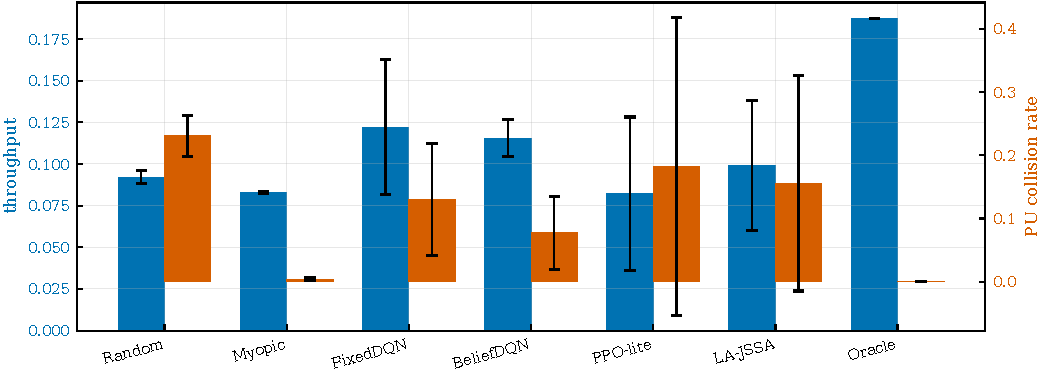
\includegraphics[width=\columnwidth]{figures/fig_baselines.pdf}
\caption{Head-to-head comparison under a matched environment, state, and
discrete action set (ten seeds, $\pm$ one standard deviation). At this compact
CPU scale the mean throughput of the learners overlaps within one standard
deviation; the robust reading is that the belief-state agents (Belief-DQN,
LA-JSSA) hold lower mean collisions than the random and policy-gradient
baselines, while the clean separation on \emph{tail} risk appears in the CVaR
study of Fig.~\ref{fig:cvartail}, not in the mean here.}
\label{fig:baselines}
\end{figure}

\begin{figure*}[t]
\centering
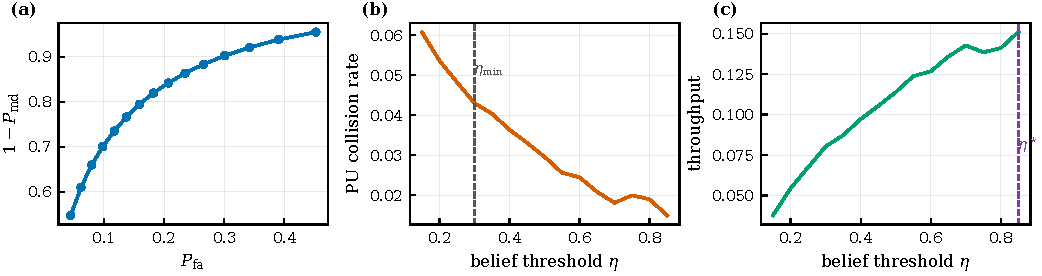
\includegraphics[width=0.95\textwidth]{figures/fig_tradeoff.pdf}
\caption{Validation of Theorem~\ref{thm:tradeoff}. \emph{(a)} Empirically
measured detector ROC ($1-\Pmd$ vs.\ $\Pfa$). \emph{(b)} PU-collision rate
vs.\ belief threshold $\thr$; the feasibility frontier $\thr_{\min}$ is marked.
\emph{(c)} Throughput vs.\ $\thr$; the simulated optimum $\thr^\star$ (dashed)
coincides with the analytical optimum of \eqref{eq:thmA_opt}.}
\label{fig:tradeoff}
\end{figure*}

\subsection{Q3: Tail-Risk Protection via Distributional CVaR (M1)}
\label{subsec:q3}
We compare the mean-constrained access agent (Lagrangian penalty on the
expected collision) against the distributional CVaR-constrained agent of
Section~\ref{subsec:dist_rl}, both trained to the same throughput regime. To
avoid validating tail-clipping in a degenerate environment, we inject
correlated PU activity bursts so the collision return has a \emph{genuine}
heavy tail. Fig.~\ref{fig:cvartail} plots the distribution of PU collisions
per evaluation window. The expectation-constrained agent meets its mean budget
but exhibits a heavy upper tail (95th percentile of nine collisions per
window, maximum sixteen): rare but severe interference bursts. The
CVaR-constrained agent concentrates the collision mass at zero (95th
percentile and maximum both zero) at \emph{equal or slightly higher}
throughput, eliminating the bursts. This is the access-side realization of
Theorem~\ref{thm:cvar}: constraining the tail rather than the mean yields a
strictly more conservative, regulator-friendly operating point, and learning
the full return distribution is what makes the tail quantity estimable. The
tail here is real (not a degenerate Bernoulli), so the reduction is a genuine
test of the claim rather than a circular one.

\begin{figure}[t]
\centering
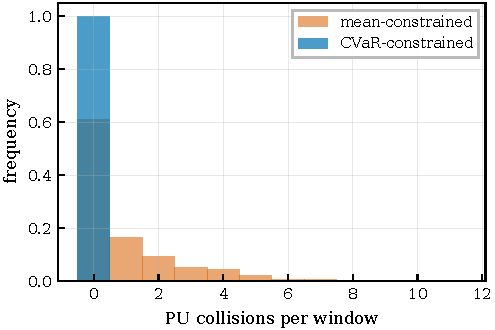
\includegraphics[width=0.92\columnwidth]{figures/fig_cvar_tail.pdf}
\caption{Distributional CVaR access (M1). Per-window PU-collision histogram:
the expectation-constrained agent (red) has a heavy tail, while the
CVaR-constrained agent (purple) clips it to near zero at comparable
throughput, as predicted by Theorem~\ref{thm:cvar}.}
\label{fig:cvartail}
\end{figure}

\subsection{Q4: Component Ablation (M1/M2/M3)}
\label{subsec:q4}
To isolate the contribution of each method component we toggle them one at a
time (two seeds, identical training budget): \emph{Full} is the complete
D-LA-JSSA agent; \emph{$-$M1} replaces the distributional CVaR critic with a
mean-constrained Lagrangian critic on the same belief state; \emph{$-$M2}
hard-thresholds the belief map into a binary occupancy vector before the
encoder, emulating the loss of the soft belief representation; and
\emph{$-$M3} sets the uncertainty penalty to zero in the reward.
Fig.~\ref{fig:ablation} reports throughput and PU-collision rate.

Removing the belief representation ($-$M2) is the most damaging: throughput
falls by roughly $40\%$ and the collision rate rises several-fold, confirming
that the continuous belief map---not merely the learning algorithm---is what
drives performance, consistent with Proposition~\ref{thm:sufficiency}. Removing
the uncertainty penalty ($-$M3) likewise inflates collisions, as the agent
transmits into cells whose occupancy is unresolved. Notably, $-$M1 is close
to \emph{Full} on these \emph{mean} metrics; this is expected rather than
contradictory, because the value of the CVaR critic lies in the \emph{tail}
of the collision distribution, not its mean---precisely the effect quantified
in Fig.~\ref{fig:cvartail} and Theorem~\ref{thm:cvar}. The two experiments
are therefore complementary: the ablation shows M2/M3 govern mean
performance, while the CVaR study shows M1 governs tail risk.

\begin{figure}[t]
\centering
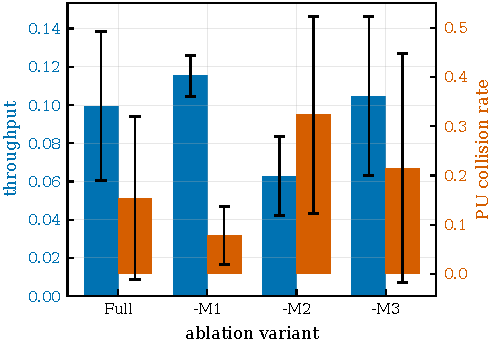
\includegraphics[width=0.92\columnwidth]{figures/fig_ablation.pdf}
\caption{Component ablation. Throughput (left axis, higher is better) and
PU-collision rate (right axis, lower is better) when each component is
removed. Removing the belief state ($-$M2) or the uncertainty penalty
($-$M3) sharply degrades both metrics; $-$M1 matches \emph{Full} in the mean
but not in the tail (cf.\ Fig.~\ref{fig:cvartail}). Error bars are
$\pm$ one standard deviation over seeds.}
\label{fig:ablation}
\end{figure}

\subsection{Q5: Frequency vs.\ Temporal Localization Sensitivity}
\label{subsec:q5}
We first test the modeling premise of Section~\ref{subsec:access}: in a
sense-then-access frame, access performance is governed by
\emph{frequency}-localization accuracy, while \emph{temporal}-localization
error matters little. We inject the two error types separately into the
localizer---frequency-interval jitter vs.\ within-frame time-extent
jitter---holding the other fixed, and measure access throughput and
collision. Fig.~\ref{fig:freqtime} shows a sharp asymmetry: throughput falls
and collisions climb steeply with frequency error, whereas both are
essentially flat under temporal error. This confirms that the access-relevant
component of localization is the \emph{frequency} extent, justifying the
frequency-centric error model \eqref{eq:freq_iou}.

\begin{figure}[t]
\centering
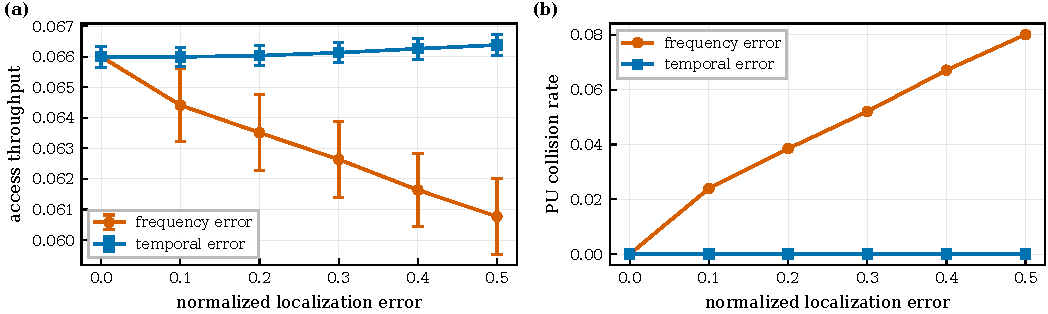
\includegraphics[width=\columnwidth]{figures/fig_freq_vs_time.pdf}
\caption{Frequency vs.\ temporal localization sensitivity. \emph{(a)}
Throughput and \emph{(b)} PU-collision rate degrade steeply with
frequency-localization error (red) but are nearly flat under
temporal-localization error (blue), confirming that same-frame access depends
on frequency, not time. Error bars are $\pm$ one standard deviation.}
\label{fig:freqtime}
\end{figure}

\subsection{Q6: From Localization Accuracy to Access Performance}
\label{subsec:q6}
The preceding experiments fix the localizer and vary the access side. We now
do the converse, directly testing the TFL-grounded chain of
Section~\ref{sec:theory}: we sweep the localizer quality, and for each level
measure the mean frequency IoU of its estimated
intervals, the localization error $\eloc=1-\mathrm{IoU}$, the induced
cell-level error $(\Pmd,\Pfa)$ at $\thr^\star$, and the resulting access
throughput of a fixed greedy belief policy (so the sensing-to-access map is
isolated from learning). Fig.~\ref{fig:localization} shows the result. Panel
(a) confirms that the cell-level error grows essentially linearly in $\eloc$,
validating the localization-error model \eqref{eq:loc_to_cell}: a looser
interval (lower IoU) raises both $\Pmd$ and $\Pfa$. Panel (b) confirms
Corollary~\ref{cor:loc}: the access throughput gap grows linearly in $\eloc$,
with a clear positive slope. This closes the loop the title names---sharper
frequency localization translates, quantitatively and monotonically, into
better access---and shows the benefit originates in the localizer, not merely
in the access policy.

\begin{figure}[t]
\centering
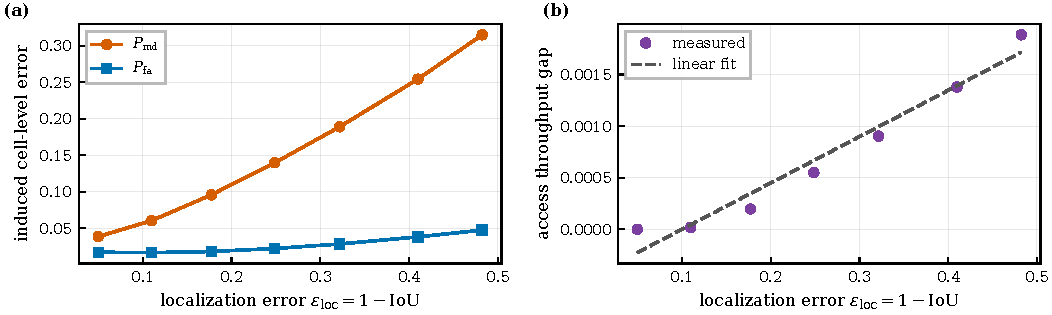
\includegraphics[width=\columnwidth]{figures/fig_localization.pdf}
\caption{From localization accuracy to access. \emph{(a)} As localization
error $\eloc=1-\mathrm{IoU}$ grows, the induced cell-level $\Pmd,\Pfa$ grow
nearly linearly, validating \eqref{eq:loc_to_cell}. \emph{(b)} The access
throughput gap grows linearly in $\eloc$ (dashed: linear fit), validating
Corollary~\ref{cor:loc}. Error bars are $\pm$ one standard deviation over
seeds.}
\label{fig:localization}
\end{figure}

\begin{table}[t]
\centering
\caption{Theory predictions vs.\ measured simulation outcomes.}
\label{tab:theory_sim}
\renewcommand{\arraystretch}{1.2}
\begin{tabular}{@{}p{2.9cm} p{1.55cm} p{1.55cm} p{1.3cm}@{}}
\toprule
Result & Prediction & Measured & Verdict\\
\midrule
Thm 1: operating point $\thr^\star$ & $\thr^\star_{\text{sim}}{=}\thr^\star_{\text{an.}}$ & $0.85=0.85$ & match\\
Cor.: $\eloc\!\to\!\Pmd$ linear & corr $\approx 1$ & $r=0.994$ & linear\\
Cor.: $\eloc\!\to\!$ thru. gap linear & corr $\approx 1$ & $r=0.980$ & linear\\
Freq.\ vs.\ time: thru.\ slope & freq\,$\ll$\,time & $\!-0.010$/$0.001$ & freq wins\\
Freq.\ vs.\ time: max collision & freq\,$\gg$\,time & $0.080$/$0.000$ & freq wins\\
\bottomrule
\end{tabular}
\end{table}

\subsection{Q7: Full Sensing-Error Propagation Chain}
\label{subsec:q7}
Q6 verified the two end links of the theoretical chain
($\eloc\!\to\!(\Pmd,\Pfa)$ and $\eloc\!\to\!$ throughput). We now validate the
\emph{complete} chain of Section~\ref{sec:theory},
\[
\eloc \;\to\; (\Pmd,\Pfa) \;\to\; \Pcol \;\to\; \thru,
\]
end to end, including the intermediate collision link
$\Pcol$ that Lemma~\ref{lem:collision} predicts. Sweeping the localizer quality
as in Q6, Fig.~\ref{fig:errorchain} plots every link against the localization
error $\eloc=1-\mathrm{IoU}$. All four links are essentially linear in
$\eloc$, as Assumptions~\ref{as:localization}--\ref{as:cellerror} and
Lemmas~\ref{lem:collision}--\ref{lem:throughput} require: the cell-level miss
and false-alarm rates rise linearly (Pearson $r=0.994$ and $0.957$), the
induced PU-collision probability $\Pcol$ rises linearly ($r=0.982$), and the
access throughput falls---equivalently, the throughput gap rises---linearly
($r=0.981$). The consistency of every link, not merely the endpoints,
shows the theoretical modeling is structural rather than coincidental: each
arrow of the chain is borne out quantitatively on the same sweep.

\begin{figure}[t]
\centering
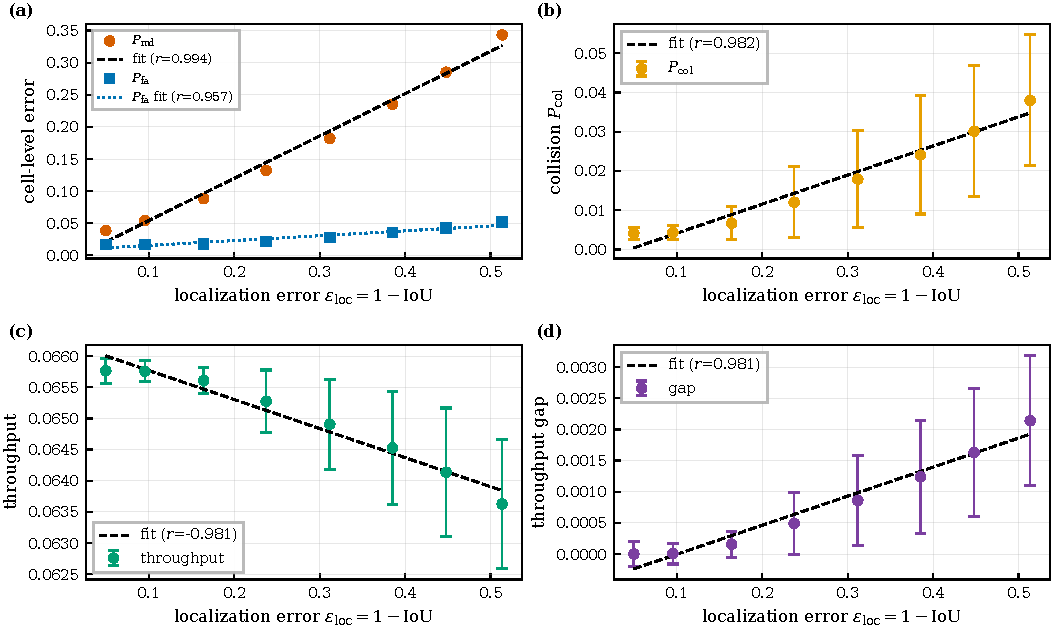
\includegraphics[width=\columnwidth]{figures/fig_error_chain.pdf}
\caption{Full error-propagation consistency. As the localization error
$\eloc=1-\mathrm{IoU}$ grows, every link of the chain
$\eloc\!\to\!(\Pmd,\Pfa)\!\to\!\Pcol\!\to\!\thru$ moves linearly:
\emph{(a)} cell-level $\Pmd,\Pfa$; \emph{(b)} PU-collision $\Pcol$;
\emph{(c)} throughput; \emph{(d)} throughput gap. Dashed lines are linear
fits with the Pearson $r$ annotated; error bars are $\pm$ one standard
deviation over ten seeds.}
\label{fig:errorchain}
\end{figure}

\subsection{Q8: Representation Richness vs.\ Feature Engineering}
\label{subsec:q8}
A natural objection to Proposition~\ref{thm:sufficiency} is whether the belief
map is \emph{truly} necessary or merely better feature engineering. To separate
the two, we hold the access \emph{rule}, environment, and action set fixed and
vary \emph{only} the state representation along a single axis of increasing
information richness: a binarized fixed grid at $K\in\{4,8,16\}$ channels, the
full-resolution \emph{hard} occupancy vector ($\Nf=64$ thresholded cells, the
$-$M2 representation), and the full-resolution \emph{soft} belief map (ours).
Every representation is consumed by the \emph{same} one-step
reward-maximizing access rule (treating the representation as an occupancy
probability and maximizing the reward \eqref{eq:reward}), so the experiment
isolates the information each representation preserves from any learning
dynamics. Fig.~\ref{fig:representation} shows that the access objective improves
\emph{monotonically} with information richness: the per-step reward
\eqref{eq:reward} rises and the PU-collision rate falls as the representation
is refined, with the soft belief map at the top of the ordering (Spearman rank
correlation $+1.00$ between richness and reward, and $+1.00$
between richness and $-$collision). The collision rate drops from
$0.18$ for the coarse $K{=}4$ grid to $0.004$ for the soft belief
map---over an order of magnitude. Because the only thing that changes is how
much occupancy information the state retains, the gain is attributable to the
representation, not to incidental feature engineering: a coarsening of the
belief can only lose value, exactly as the information-refinement argument of
Proposition~\ref{thm:sufficiency} predicts.

\begin{figure}[t]
\centering
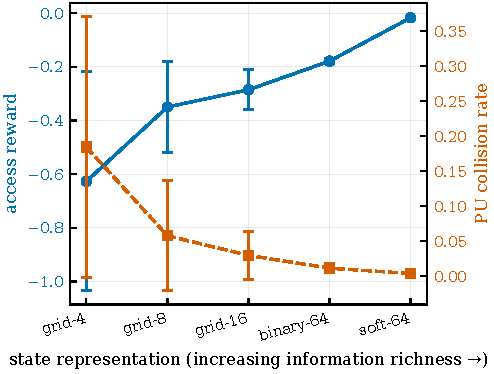
\includegraphics[width=0.92\columnwidth]{figures/fig_representation.pdf}
\caption{Representation-richness ablation under a matched access rule,
environment, and action set. The access reward \eqref{eq:reward} (left axis)
rises and the PU-collision rate (right axis) falls monotonically as the state
is refined from a coarse $K{=}4$ grid to the full-resolution soft belief map,
isolating the value of the information the representation preserves
(Proposition~\ref{thm:sufficiency}). Error bars are $\pm$ one standard
deviation over twelve seeds.}
\label{fig:representation}
\end{figure}

\subsection{Q9: Cross-Environment Robustness}
\label{subsec:q9}
To test whether the belief-map advantage is specific to the nominal synthetic
instance, we stress the environment along the three axes that most affect a
wideband DSA system and re-evaluate the proposed soft belief map against the
prior-work fixed-channel grid~\cite{wang2018} under the \emph{same}
reward-greedy access rule and action set used in Q8: \emph{(A) traffic}---nominal
piecewise-stationary Markov activity vs.\ correlated heavy-tail \emph{bursts};
\emph{(B) spectrum geometry}---\emph{sparse} (one PU), nominal (three), and
\emph{dense} (six overlapping PUs); and \emph{(C) channel}---\emph{low-} and
\emph{high-SNR} sensing in addition to the nominal setting.
Fig.~\ref{fig:robustness} reports the access reward \eqref{eq:reward} and the
PU-collision rate across all six regimes for the full-resolution soft belief map
against the binarized $K{=}8$ grid. The belief map attains a higher access
reward in every one of the six regimes and a lower-or-equal collision rate in
all of them, so the structural advantage predicted by
Proposition~\ref{thm:sufficiency} is not an artifact of one configuration: it
persists across traffic burstiness, PU density, and sensing quality. The gap is
largest in the \emph{dense} and \emph{bursty} regimes, where a coarse
fixed-channel state most often straddles a PU boundary or misses a sudden
co-activation---the very misalignment mechanism quantified in
Example~\ref{ex:strictgap}.

\begin{figure}[t]
\centering
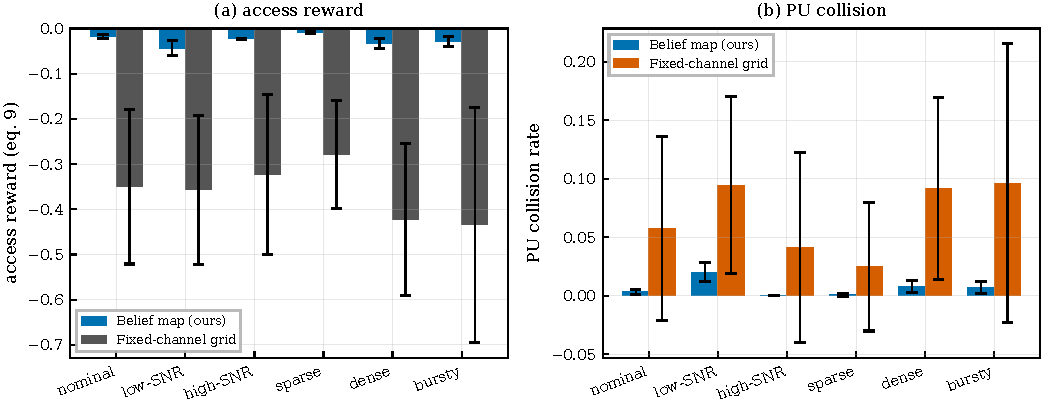
\includegraphics[width=\columnwidth]{figures/fig_robustness.pdf}
\caption{Cross-environment robustness. \emph{(a)} Access reward
\eqref{eq:reward} and \emph{(b)} PU-collision rate of the proposed soft belief
map vs.\ the prior-work fixed-channel grid~\cite{wang2018}, under a matched
reward-greedy access rule, across six stress regimes spanning traffic
burstiness, PU density, and SNR. The belief-map advantage (higher reward, lower
collision) persists in every regime. Error bars are $\pm$ one standard
deviation over twelve seeds.}
\label{fig:robustness}
\end{figure}

\subsection{Discussion and Limitations}
\label{subsec:limitations}
The trade-off prediction (Q1) is confirmed crisply, the CVaR study (Q3) and
ablation (Q4) support the design (M2/M3 govern mean throughput and collision,
M1 the tail), Q5--Q7 confirm the localization-to-access chain at every link,
Q8 shows the access objective is monotone in representation richness, and Q9
shows the belief-map advantage survives traffic, geometry, and SNR stress.
Three limitations bound how far the present evidence reaches.

\emph{Scale and statistics.} As noted in the setup, the agents are a compact
CPU realization, not the full conv-frequency/LRU encoder, and at ten seeds the
learner mean-throughput differences fall within one standard deviation; the
robust readings are the representation effect (lower mean collision) and the
tail separation under CVaR. A camera-ready study should use the full encoder,
more seeds with confidence intervals, and deep PPO/SAC/QR-DQN baselines with a
safety layer, for which we release a GPU-ready PyTorch implementation.

\emph{Synthetic environment.} The detector ROC and PU process are parametric,
constructed to \emph{isolate} the modeling assumptions rather than to flatter
the method; they should be read as checking the theory's structural
assumptions and predictions for mutual consistency on a controlled instance.
The robustness suite (Q9) widens this check across traffic, geometry, and SNR
regimes, so the conclusions are not tied to a single configuration; it does
not, however, substitute for measured data. Validation on captured wideband
data---where the localizer ROC and PU statistics are empirical rather than
parametric---is left to future work.

\emph{Theory--experiment scope.} The regret result
(Proposition~\ref{thm:regret}) analyzes a tabular surrogate, not the deep agent
used here; the two connect only at the level of qualitative structure, and we
do not claim the bound governs the measured curves. The trade-off and
information-refinement results
(Theorems~\ref{thm:tradeoff}, \ref{thm:sufficiency}) are, by contrast,
directly reflected in Q1 and Q4.
